\section{OR-Mapper}

    \subsection{Klasse mit Annotation \@Entity}
        \begin{itemize}
          \setlength{\itemsep}{0pt}
          \item Kann erben und vererben
          \item Kann Interfaces implementieren
          \item Kann abstrac seien
        \end{itemize}
    \begin{multicols}{2}   
    \subsection{Laden/Suchen von Entities}
    
\begin{lstlisting}[style=Java] 
EntityManagerFactory factory =
    Persistence.createEntityManagerFactory("Bank");
EntityManager em = factory.createEntityManager();
Query query = em.createQuery("SELECT a FROM BankAccount a");
List<BankAccount> list = query.getResultList();
for (BankAccount account : list) {
    System.out.println(account);
}
em.close();
\end{lstlisting}
    
    \subsection{Table/Cloumn Mapping}
        
\begin{lstlisting}[style=Java]
@Entity
//Name der DB-Tabelle
@Table(name = "Account") 
public class BankAccount {
    @Id
    //Name der DB-Column
    @Column(name = "AccountId")
    private long id;
    //Automatisch 1:1 Mapping
    private double balance;
    @Column(name = "description")
    private String explanation;
    \\ Zusatzinformation fuer DATE/TIME-Typen
    @Temporal(TemporalType.TIMESTAMP)
    private Calendar creationDate;
    \\Nicht Persistent
    @Transient nicht in DB
    private String tempComments;
\end{lstlisting}
        
    \subsection{Entity Relations}
        \subsubsection{OneToOne (1:1)}
\begin{lstlisting}[style=Java]
@OneToOne(optional = true)
@JoinColumn(name = "addressref")
private Address address;
\\Bidirektional
class Address {
    @OneToOne(mappedBy="address")
    private BankCustomer customer;}
\end{lstlisting}
        \subsubsection{OneToMany (1:N)}
\begin{lstlisting}[style=Java]
@OneToMany
@JoinColumn(name = "CustomerRef",
    referencedColumnName="CustomerId")
private Collection<BankAccount> accounts = ...
\end{lstlisting}
        \subsubsection{ManyToOne (N:1)}
\begin{lstlisting}[style=Java]
class BankAccount { 
    @ManyToOne(optional = false) 
    @JoinColumn(name = "CustomerRef") 
    private BankCustomer customer;}
\\Bidirektional
@OneToMany(mappedBy = "customer")
private Collection<BankAccount> accounts = new ...
\end{lstlisting}
        \subsubsection{ManyToMany (M:M)}
\begin{lstlisting}[style=Java]
class BankManager { 
    @ManyToMany @JoinTable(name = "Customer_Manager", 
        joinColumns = {@JoinColumn(name = "CustomerRef")}, 
        inverseJoinColumns = {@JoinColumn(name = "ManagerRef")}) 
    private Collection<BankCustomer> customers = ...
\\Bidirektional
class BankCustomer {
    @ManyToMany(mappedBy = "customers")
    private Collection<BankManager> managers = new ...
\end{lstlisting}
    \subsection{Laden der Relations}
\begin{lstlisting}[style=Java]
Query query = em.createQuery("select a from BankAccount a");
List<BankAccount> accountList = query.getResultList();
for (BankAccount account : accountList) {
    BankCustomer customer = account.getCustomer();
    for (BankManager manager : customer.getManagers()) {
        ...}
}
\end{lstlisting}
    \end{multicols}
    
    \subsection{JPA Architektur}
        \includegraphics[page=7,trim=50 40 0 90,clip=true,width=0.7\textwidth]{images/or-mapping_fortsetzung.pdf}                